\subsection{Case Study}
\label{sec:case-study}

We use an illustrative case to show how the system combines capabilities from different Skills, fills missing steps, and forms concrete tool calls. Consider the task: given several remote-sensing rasters of the same region, create and return a pixel-wise mean composite, compute the mean of its valid pixels, state whether that mean exceeds a given reference value, and report the difference. The inputs represent the same variable, their spatial grids are aligned, and the reference value uses the same units as the raster values.

\begin{figure*}[t]
  \centering
  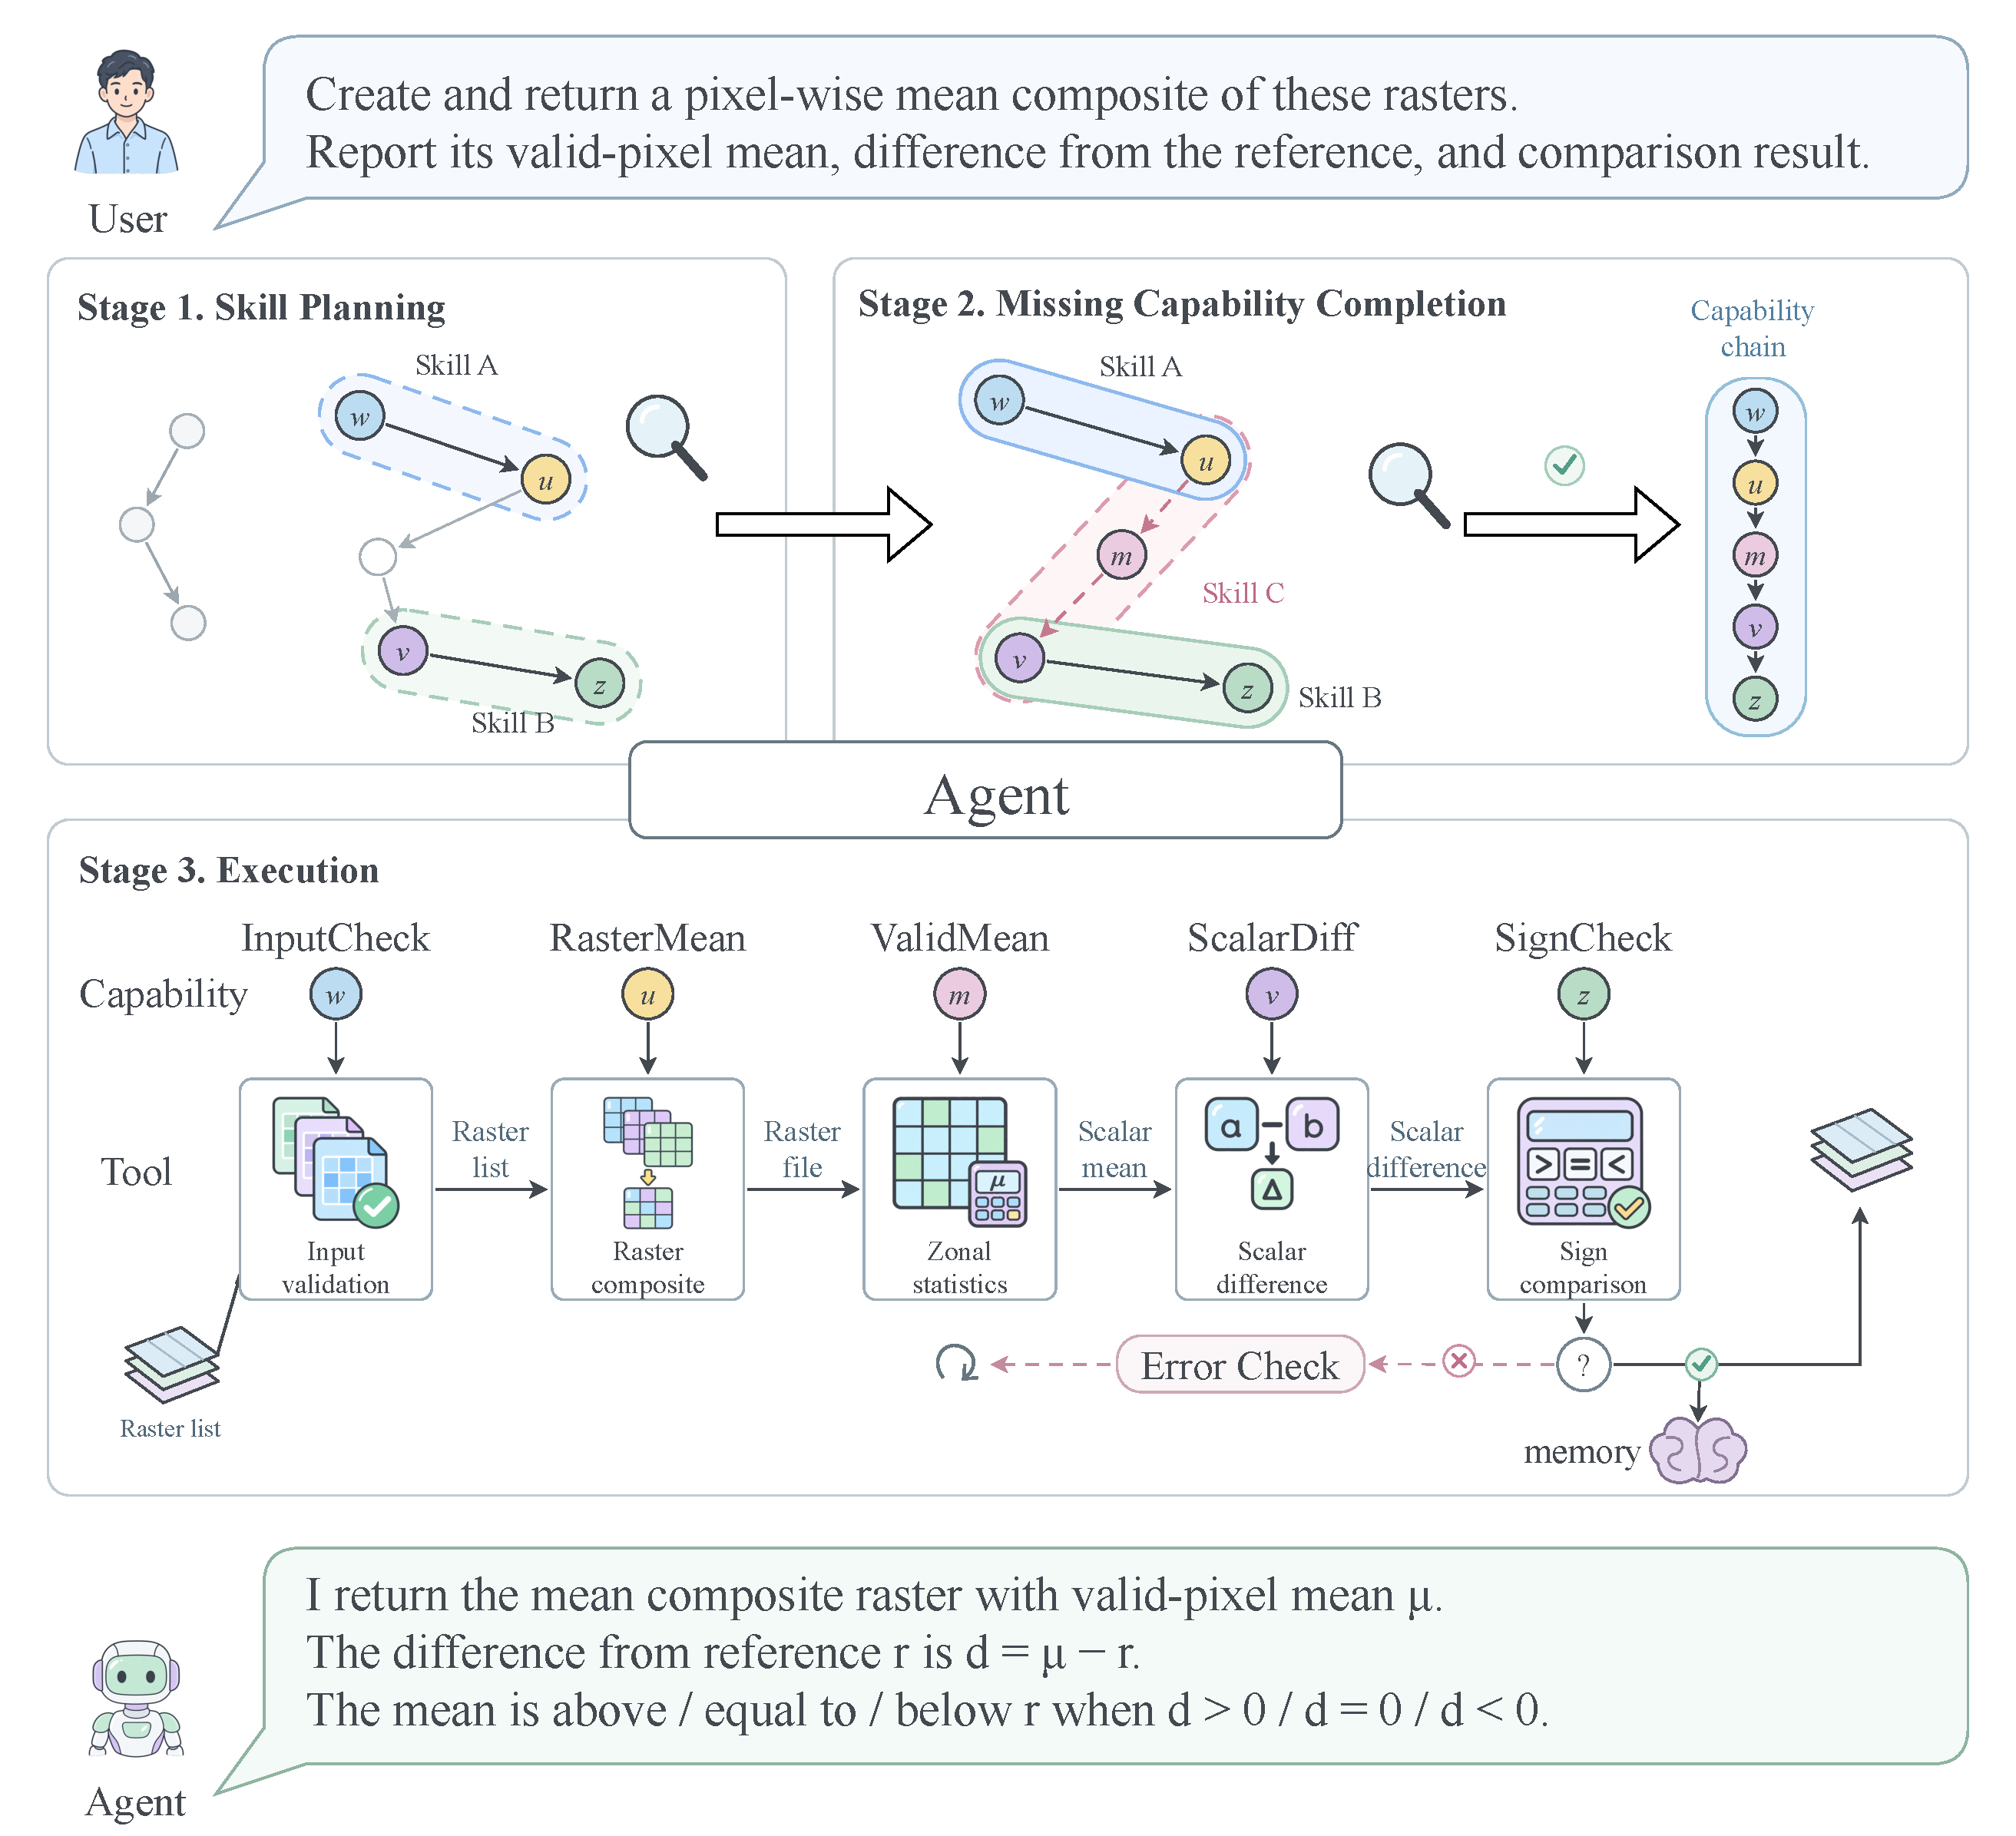
\includegraphics[width=0.83\textwidth]{fig_case_study.pdf}
  \caption{Cross-Skill capability composition and tool execution. Stage 1 selects $w\to u$ from Skill $A$ and $v\to z$ from Skill $B$. Stage 2 inserts valid-pixel mean statistics $m$ using Skill $C$'s $u\to m\to v$ branch. Stage 3 grounds the five-step workflow in tool calls, propagates intermediate artifacts, and returns the composite raster, mean, difference, and comparison relation. The workflow is a mechanism illustration.}
  \label{fig:case-study}
  \Description{The case proceeds from two selected Skill fragments to a completed five-capability chain and corresponding input-validation, raster-compositing, zonal-statistics, scalar-differencing, and sign-comparison tools.}
\end{figure*}


\emph{Skill Retrieval} returns only RasterCompose (Skill $A$) and ReferenceCompare (Skill $B$). \emph{Skill Planning} selects InputCheck ($w$) and RasterMean ($u$) from the former, and ScalarDiff ($v$) and SignCheck ($z$) from the latter. InputCheck verifies the variable and spatial-grid requirements. RasterMean produces the mean raster from the validated image list, giving $w\to u$. ScalarDiff returns the difference between the value under comparison and the reference; SignCheck uses that difference to determine whether the value is above, equal to, or below the reference, giving $v\to z$. Hypergraph Composition expands mandatory predecessors declared by the selected strategies and retains provenance and candidate-tool scopes. At this stage, the plan consists of two disconnected fragments: compositing produces a raster file, whereas differencing requires a numerical input. The operation computing the mean of the composite is still missing.

Using $u$ and $v$ as shared endpoints, Missing Capability Completion retrieves $u\to m\to v$ from inactive RasterDiff (Skill $C$), where ValidMean ($m$) extracts the mean of valid pixels from the composite. Here, RasterDiff means differencing a statistic of the composite against a reference value. The query explicitly requires the mean statistic; Skill $C$ supplies reusable dependencies and usage constraints connecting it to the preceding and following operations. Under this example's assumptions, it is the only candidate for the ordered endpoint pair satisfying prerequisite, type, tool-availability, and acyclicity requirements: $u$'s raster output is compatible with $m$'s input, and $m$'s numerical output is compatible with $v$. Insertion preserves $u$'s original constraints, adds $m$, and updates $v$'s dependencies, candidate-tool scope, and input bindings. Existing dependencies $w\to u$ and $v\to z$ remain. Recomposition and dependency verification connect the fragments into input validation, mean compositing, valid-pixel mean statistics, scalar differencing, and sign comparison: $w\to u\to m\to v\to z$.

Tool Grounding then selects validation, compositing, statistics, differencing, and sign-comparison tools within each instance's candidate scope and parameter constraints. GeoToolKG associations guide candidate retrieval, but concrete invocations still require instance and input-compatibility checks. Grounding a bridge into calls additionally requires that $u$ and $v$ each correspond to exactly one endpoint instance and that their order agrees with the bridge direction. During execution, the validated image list is passed to the compositing tool. The statistics tool receives a list containing only the composite raster's path. The returned mean and the task's reference value are bound to differencing parameters $a$ and $b$, producing $d=a-b$. Sign comparison then compares $d$ with zero. The statistical object remains the composite created for this task, the comparison baseline remains the supplied reference, and the final relation is based on the same difference calculation.

If the zonal-statistics call fails, Failure Recovery uses the failure state and recovery rules to decide whether to retry or select an alternative within the instance's permitted scope. Completed validation and compositing steps are retained, and the composite is reused. Calls with uncertain outcomes are not automatically replayed, and later execution is suspended if recovery requires adding a capability. Once all steps succeed, Final Answer summarizes the composite raster, valid-pixel mean, difference, and comparison relation, addressing each requested output. This case illustrates that cross-Skill completion must both connect capability steps and preserve dependencies while accurately binding task inputs and intermediate artifacts to subsequent calls.

After successful execution and result verification, the five-step workflow can also be organized into a candidate CompositeCompare Skill ($D$). It parameterizes the image list and reference value as rebindable task inputs, and retains artifact dependencies and capability usage constraints. This provides a strategy description for later reuse of the composition. Applicability to other inputs and tasks requires further verification; the example does not establish a reuse benefit for the new Skill.
